% !TEX root = ../my-thesis.tex
%
\chapter{Related Work}
\label{sec:related}

\cleanchapterquote{A picture is worth a thousand words. An interface is worth a thousand pictures.}{Ben Shneiderman}{(Professor for Computer Science)}





\section{Introduction}
\label{sec:related:sec1}
Depth perception is the ability to visually perceive the world around us in 3-dimensions. Although such depth perception is an ambiguous and a very ill posed problem, humans are able to recognize certain patterns and cues in the perceived visual stimulus and thus comprehend the  3-dimensional surroundings. 
This chapter begins with a brief glimpse of how depth perception manifests in humans and further sections describe the various techniques of depth estimation in computer vision.  

In human vision, various sensory stimuli present in the  2-dimensional retinal images provide information that contributes to the depth perception of the surroundings.
Research conducted in \cite{koenderink1998pictorial} suggests that depth perception is closely connected to object identification.
Consider figure \ref{fig:ireland-g77640d1c91280} and order different levels of depth in the image. Most people would suggest that the \textit{person} is in front of the \textit{lake} and that the \textit{lake} is in front of the \textit{mountains} and that the \textit{mountains} are in front of the \textit{sky}. This suggests that humans perceive a 3-dimensional scene not in terms of a depth map but rather in terms of distinct objects that are spatially oriented.
Although humans, learn such a spatial ordering through experiences in their lifetime, there are certain patterns or cues in images which hints a discontinuity or variation in depth. Research by Cutting and Vishton \cite{cutting1995perceiving} suggests that to perceive depth of objects closer that $ 30m $, binoucular and motion cues play an important role whereas for objects beyond $30m$, pictorial cues that are monocular, turn out to be beneficial.


\begin{figure}[h]
	\centering
	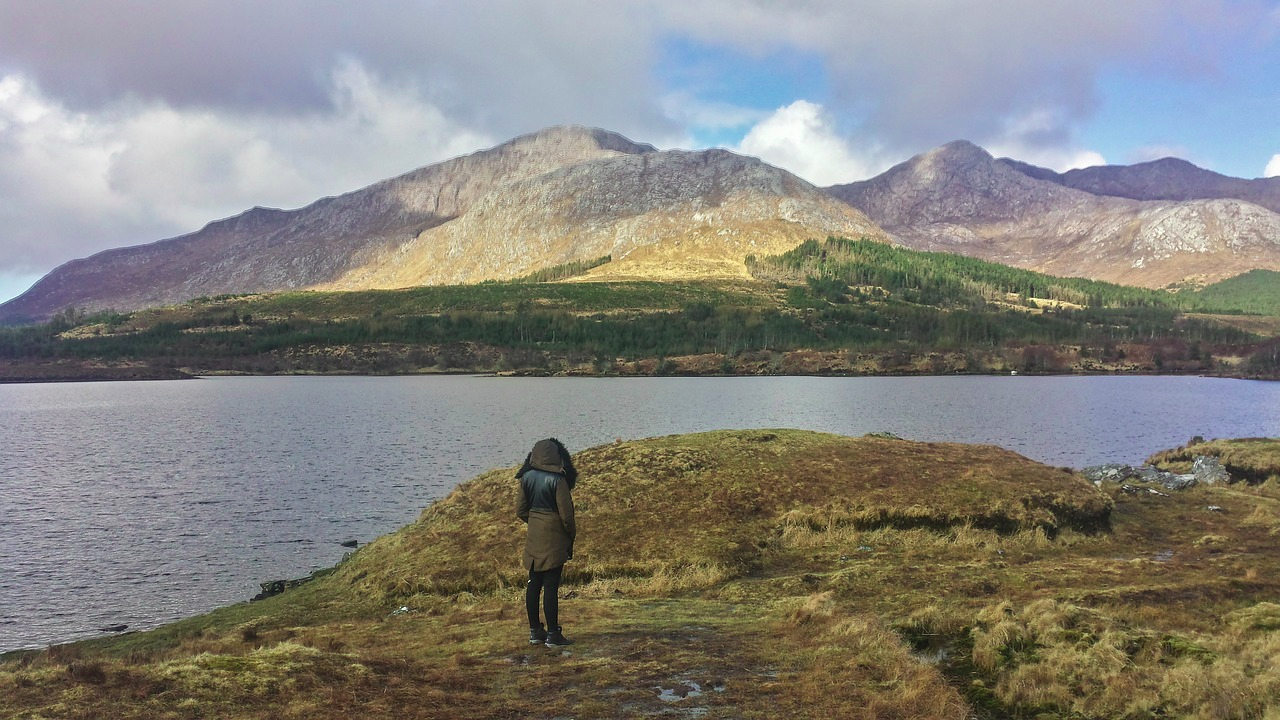
\includegraphics[width=\textwidth]{content/imgs/ireland-g77640d1c9_1280}
	\caption{Example illustrating how human vision identifies objects in the image and then orient them spatially}
	\label{fig:ireland-g77640d1c91280}
\end{figure}

Studies described by Marko Teittinen in \cite{teittinen1993depth} show that there are several pictorial cues supporting depth perception. Each of them are described below:
\begin{itemize}
	\item \textbf{Occlusion} : An occlusion is a phenomenon where one object partially covers another object in sight. The occluded object appears to be further and hence provides information of the depth order in the scene. 
	
	\item \textbf{Linear Perspective} : This is a result of perspective projection. Parallel lines appear to converge towards a vanishing point as they travel into the distance.
	
	\item \textbf{Relative and familiar size} : Given 2 objects of equal or known sizes, the one at a farther distance appears smaller than the one closer. This phenomenon is also a result of perspective projection. However a prior information regarding the objects is necessary to make such inferences.
	
	\item \textbf{Texture gradients} : The patterns in the texture and their sharpness vary with distance. Farther objects have a smoother fine texture whereas when the same object is near, it contains a richer and well defined texture.
	\item \textbf{Monocular Movement Parallax} : An object can be perceived from two different positions and the minor disparity in the two perceptions can be useful to extract depth. 
\end{itemize}

In the 1980's it was the experiments conducted by Marr \cite{marr1979computational} that developed computer vision methods to reconstruct 3D representation from 2D images. This found popularity in various artificial intelligence applications in computer vision. In computer vision, there are two prevalent methodologies for depth estimation. The first one being monocular depth estimation and the second id Depth from stereo images. Further sections describe various techniques used in these depth estimation methods. 

\section{Stereo Depth Estimation} 
\label{sec:related:sec2}
In stereo vision based depth estimation, the system analyses two or more images of the same scene and learns a mapping from the disparity in the two images to 3D depth. Stereo depth estimation is comprised of two tasks \cite{li2021revisiting}:
\begin{enumerate}
	\item Feature matching in the stereo images.
	\item Optimizing the matched cost aggregation.
\end{enumerate}
Traditional methods achieved this using dynamic programming techniques where feature matching is computed using using pixel intensities and then aggregating the costs either along one direction or along multiple directions in 2D \cite{li2021revisiting}. 
Further, learning based methods where features were learnt instead of manually coded emerged. Such methods matched features using correlation techniques and further refined the matching using Markov Random Field \cite{2020}.


Convolutional neural networks(CNN) have been shown
to perform very well on high-level vision tasks. More recently, CNNs have been applied to low-level
vision tasks such as optical flow prediction \cite{Luo_2016_CVPR}. In the context of stereo estimation, Techniques by Yann LeCun et al. \cite{2015} utilize CNN to compute the
matching cost between two image patches. The cost is refined by cross-based cost aggregation and semi-global matching, followed by a left-right consistency check to eliminate errors in the occluded regions \cite{2015}. The  model was trained to minimize a binary cross-entropy loss\cite{Luo_2016_CVPR}.
Other approaches like \cite{guo2019group} combine 3D convolutions and correlation methods for cost aggregation and feature matching respectively.
Recent work on stereo matching trained on large datasets  compute features, their similarity cost and can regularize the cost volume within a single end-to end trained model. Work presented in \cite{li2021revisiting}, utilize vision transformer architecture to produce an end-to-end depth estimation network named STereo TRansformer (STTR). This method is more advanced in the sense that it uses a Transformer to compute pixel wise correlation in a dense manner without building a fixed-disparity cost volume \cite{li2021revisiting}.


\section{Monocular Depth Estimation}
\label{sec:related:sec3}
Monocular Depth Estimation(MDE) is the process of estimating a dense depth map for a given RGB image captured from a single camera. More specifically, a depth value, either metric or relative depth, must be estimated for every pixel/segment in the given image. There exists numerous techniques to achieve this in literature based on the underlying requirement. Broadly it can be classified as metric depth estimation: where the estimated depth map consists of accurate metric depth and ordinal depth estimation: where the predicted depth map consists of relative depth information only. Further sections describe each of these methods in more detail.
\begin{figure}[h]
	\centering
	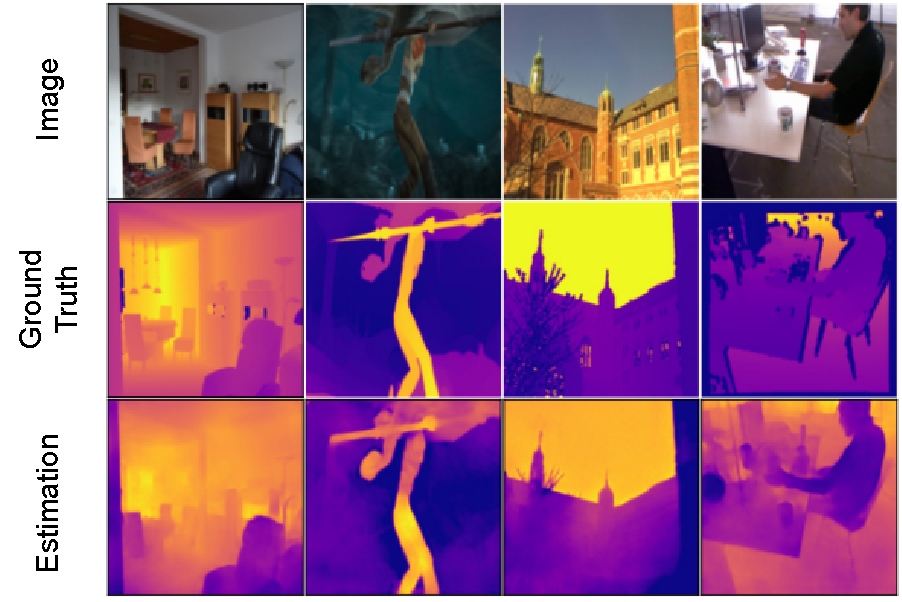
\includegraphics[width=\textwidth]{content/imgs/mde_img.drawio}
	\caption{An example of monocular depth estimation. The estimated depth is predicted from PLDepthEffNet model described in \cite{Lienen_2021_CVPR}. Source:\cite{Lienen_2021_CVPR}}
	\label{fig:mdeimg}
\end{figure}

\subsection{Metric Depth Estimation}
\label{sec:related:sec3:subsec1}
%Experiments conducted by Saxena \textit{et al.}\cite{saxena2005learning} are one of the first studies using Markov Random Field(MRF) to predict depth from monocular images. Since then, various deep neural network(DNN) based methods have been introduced.
%Training large RGB datasets on deep learning based CNNs have resulted in commendable performance in monocular depth estimation. Typically, it was solved as a regression problem in a supervised learning format. In \cite{eigen2014depth}, metric depth is regressed using a CNN in two stages. The first stage estimates the global structure of the scene and the second refines it using local information. In the works of Liu \textit{et al.}\cite{liu2015learning}, a deep convolutional neural field model was proposed which combines CNN models with continuous conditional random field(CRF). Furthermore, attention models that were previously used in natural language processing was introduced in monocular depth estimation. Huynh \textit{et al.}\cite{attention} devised depth-attention volume model which enhanced depth estimation by capturing non-local depth dependencies between co-planar points. The contemporary state of the art method is based on vision transformers. \cite{ranftl2021vision} proposed dense prediction transformers(DPT) for monocular depth estimation which results in more fully grained coherent predictions when compared to CNN based architectures. 
%In contrast to supervised learning methods, \cite{10.1007/978-3-319-46484-8_45} predicts a depth map using unsupervised learning techniques. Recent works by Zhu \textit{et al.}\cite{zhu2020edge} utilize the border constraint between semantic segmentation and depth estimation such that the inconsistency between the segmentation edge and the depth edge is used as the loss function. 


\subsubsection*{Supervised Learning Methods}
\label{sec:related:sec3:subsec1:part1}
Experiments conducted by Saxena \textit{et al.}\cite{saxena2005learning} are one of the first studies using Markov Random Field(MRF) to predict depth from monocular images in which the modelling of global context information was implemented using manually
engineered features. In \cite{4408828} Saxena \textit{et al.} developed a framework to estimate 3D structure from an unstructured environment via the superpixel segments. The environment was assumed to be made of successive planar surfaces and each superpixel was assumed to lie on one planar surface. The MRF was trained in a supervised learning fashion to learn the monocular depth cues. Since then, various deep neural network(DNN) based methods have been introduced.\\
Training large RGB datasets on deep learning based CNNs have resulted in commendable performance in monocular depth estimation. Typically, it was solved as a regression problem in a supervised learning format. Eigen \textit{et al.} \cite{eigen2014depth} developed a technique where metric depth is regressed using a CNN in two stages. The first stage estimates the global structure of the scene and the second refines it using local information. The training cost function used the experiment is defined as:
\begin{align*}
	L(d,d^*) = \frac{1}{N} \sum_{i}^{N} y_i^2 - \frac{\lambda}{N^2} \left( \sum_{i}^{N}y_i\right)^2 
\end{align*}
where $ d^{*} $ is the true depth, $ d $ is the predicted depth, $ y_{i}^2 = \log(d) - \log(d^{*}) $ and $ \lambda \in [0,1]$ is called the balance factor that controls scale invariance \cite{eigen2014depth}.
In the works of Liu \textit{et al.}\cite{liu2015learning}, a deep convolutional neural field model was proposed which combines CNN models with continuous conditional random field(CRF). Furthermore, attention models that were previously used in natural language processing was introduced in monocular depth estimation. Huynh \textit{et al.}\cite{attention} devised depth-attention volume model which enhanced depth estimation by capturing non-local depth dependencies between co-planar points.\\\\
Due to the superior demonstrated performance of ResNet \cite{7780459} in image recognition, Laina \textit{et al.} \cite{laina2016deeper} developed a ResNet based model that maps RGB image pixels to the corresponding depth. Moreover, the final resolution of the predicted depth map was better owing to the fact that the up-sampling blocks were used in the ResNet instead of a fully connected layer. Here, the BerHu loss(inverted Huber) was used as the optimization criterion. It is defined as follows:
\begin{align*}
	L_{BerHu}(d, d^{*}) = \begin{cases}
		|d-d^{*}|,  & if |d-d^{*}| < c \\
		\frac{(d-d^{*})^2 + c^2}{2c}, &if |d-d^{*}| \geq c
	\end{cases}
\end{align*}
where $ d^{*} $ is the true depth, $ d $ is the predicted depth and $c$ is a threshold chosen to be $\frac{1}{5} \max(|d-d^{*}|)$

The contemporary state of the art method is based on vision transformers. \cite{ranftl2021vision} proposed dense prediction transformers(DPT) whose backbone is based on dense vision transformers in place of convolutional neural networks for dense prediction in monocular depth estimation. This trains the monocular depth estimation network using a scale and shift-invariant trimmed loss that operates on an inverse depth representation, together with
the gradient-matching loss \cite{ranftl2021vision}.  This results in more fully grained coherent predictions when compared to CNN based architectures. 

\subsubsection*{Unsupervised Learning Methods}
\label{sec:related:sec3:subsec1:part2}

In contrast to using ground truth depth data for supervising the training, these methods use the epipolar geometry(similar to methods described in \ref{sec:related:sec2}) present between the left and right pairs of images as their supervisory signal.
\begin{figure}[h!]
	\centering
	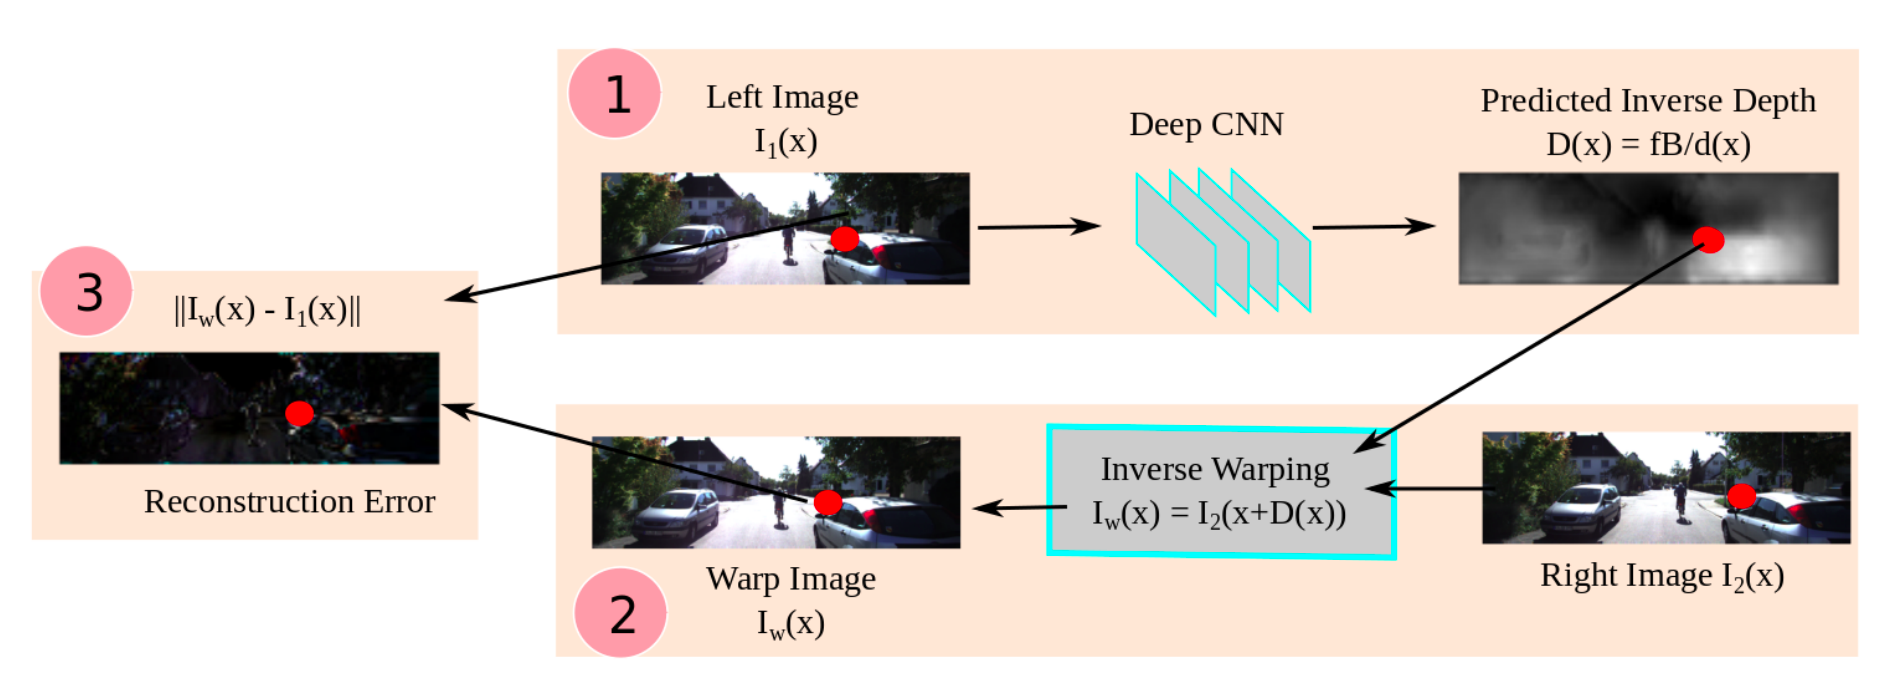
\includegraphics[width=\linewidth]{content/imgs/unsup}
	\caption{Summarizing the Unsuperviled Monocular Depth Estimation process employed in \cite{10.1007/978-3-319-46484-8_45}. Source: \cite{10.1007/978-3-319-46484-8_45}}
	\label{fig:unsup}
\end{figure}


 As one of the first work using this approach, Garg \textit{et al.} \cite{10.1007/978-3-319-46484-8_45} predicts a depth map using unsupervised learning techniques. They utilized an end-to-end auto-encoder network where the convolutional network encodes the input image into a depth map and then inversely warps the other image of the pair using the depth map with a reconstruction minimization loss as described in Figure \ref{fig:unsup}.
 Godard \textit{et al.} \cite{godard2017unsupervised} further improve the method in \cite{10.1007/978-3-319-46484-8_45}. They train their network with rectified stereo pairs to estimate disparity maps ($ Disp\_left , Disp\_right $). Having left and right
 disparity maps made it possible to reconstruct both of the images within the pair to derive better estimates.
 \begin{align*}
 	I_{left}(Disp_right)~ I_{right}, \quad I_{right}(Disp_left)~ I_{left}
 \end{align*}
 where $ I_{right} $ and $ I_{left} $ are the input image pairs \cite{mertan2021single}.
 
Another prominent work that solves the depth estimation problem in an unsupervised manner is the work of Zhou \textit{et al.} \cite{Zhou_2017_CVPR}. In this work, the network is trained on datasets comprised of video recordings obtained by a single camera. Subsequent frames are used to train the network by utilizing the small camera position  disparity between them which act like a stereo pair. In contrast to the work of Garg \cite{10.1007/978-3-319-46484-8_45} and Godard \cite{godard2017unsupervised}, the camera position is unknown. Therefore, a separate network is trained to estimate the camera position. Hence, a video from any source can be used as the data input.

Such a multi-view  reconstruction between successive video frames assume that the object position in the two frames do not change. However, this is not the case in real-world data. In order to address this issue, a
mask to minimize the effect of dynamic objects present in the scene is necessary. Vijayanarasimhan \textit{et al.} \cite{vijayanarasimhan2017sfmnet}  designed an object mask network to model the dynamic objects present in the
scene. Dense optical flow mask is predicted on these images and differentiably warps frames in time to match pixels and back-propagates. However, such an approach increases the computation cost and makes the training difficult. 
As a further improvement to reduce the load on the network, Bian \textit{et al.} \cite{bian2019unsupervised}  used geometry-based masks instead of estimating it by the deep neural network. This replacement improved the performance of the model.
Additionally, recent work by Zhu \textit{et al.}\cite{zhu2020edge} utilize the border constraint between semantic segmentation and depth estimation such that the inconsistency between the segmentation edge and the depth edge is used as the loss function.
\subsection{Ordinal Depth Estimation}
\label{sec:related:sec3:subsec2}
Using relative depth The term ”relative depth” refers to the ordering of the depth of pixels instead of absolute depth which refers to the metric depth values. Relative depth can be used to
measure the performance of the system or can be used as an error function. This way, the system would not be penalized for mistakes due to scale ambiguity.
\subsubsection*{Ranking Methods}
\label{sec:related:sec3:subsec2:part1}
Learning to rank is a popular machine learning technique used in Information Retrieval(IR)\cite{cao2007learning}. The task of such models is to construct a ranking model using training data, such that it can sort new samples based on their degree of preference.
Ranking methods mainly fall under two categories: pair-wise methods and list-wise methods. For a given query, pair-wise methods order/classify a pair of samples according to its importance. It is trained using a pair-wise loss function as in \cite{chen2016single}. A query in list-wise method consists of a list of samples and the method sorts the elements of the list according to a degree of preference. List-wise methods define losses over the set of permutation of the samples in the list \cite{liu2011learning}. It has been observed that list-wise methods yield a better performance than pairwise ranking methods \cite{cao2007learning}.


\subsection*{Depth Estimation}
\label{sec:related:sec3:subsec2:part2}
Certain applications like 2D-to-3D conversion and depth-of-field do not demand the exact metric depth prediction. Models for such applications can be trained on pseudo-depth information. Such models can be designed as ranking models described above, which rank pixels/objects based on their pseudo depth.  Zoran \textit{et al.}\cite{zoran2015learning} uses a CNN model that is trained on pseudo-depth samples taken pair-wise on the basis of superpixel segmentation and later derives a global depth map by solving an energy optimization problem. Further, Chen \textit{et al.}\cite{chen2016single} proposed a "Depth in the Wild"(DIW) dataset with images containing manually annotated sample point pairs with their relative depth. A CNN model was trained with this data by minimizing a ranking loss function to predict a dense metric depth map. However, the DIW dataset only provides labels for only one pair of points in every image, hence missing out on a large amount of perception relevant information. 
To overcome this drawback, Xian \textit{et al.}\cite{xian2018monocular} introduced a method to automatically produce dense relative depth annotations from web stereo images. Now, multiple sample pairs were randomly sampled in order to train a ResNet based CNN model to minimize an improved ranking-loss function. Chen\textit{ et al.}\cite{chen2019learning} proposed a method to automatically generate monocular depth data by integrating structure from motion(SfM) and a quality assessment network.  
In the depth estimation methods described so far, training sample pairs were sampled randomly from images without considering depth cues or structure in the image which contains higher information and have the potential to yield a better performance in depth estimation. In this regard, Xian \textit{et al.}\cite{xian2020structure} proposed a novel structure guided sampling technique. The authors stated that samples in the image across edges and segments contain higher structural information and are hence, more relevant in depth prediction. Therefore, the ResNet50 based model was trained on such selective samples to minimize a novel structure guided ranking-loss\cite{xian2020structure}. 

Relative depth prediction models trained on pair-wise samples in \cite{zoran2015learning,chen2016single,xian2018monocular,xian2020structure} have proven to be effective. These models solve depth estimation as a pair-wise ranking problem by reducing a pair-wise ranking loss function. However, the fact that a large number of sample pairs can be constructed, renders these methods to be rather inefficient. 
In order to overcome this problem, list-wise ranking \cite{xia2008listwise} was introduced as an alternate to pair-wise ranking. The inherent feature of list-wise ranking is that, it allows for higher order ranking of arbitrary length data to be training samples. It is also demonstrated that list-wise ranking yields higher performance than pairwise ranking \cite{xia2008listwise}.

Monocular relative depth estimation was formulated as a list-wise ranking problem in \cite{Lienen_2021_CVPR}. Training samples were sampled randomly as lists and trained on PLDepthEffNet model \cite{Lienen_2021_CVPR} by optimizing the ListMLE loss function\cite{xia2008listwise}. In ListMLE, the permutations of the list is modeled as a probability distribution using the Plackett Luce model. The ListMLE loss is the negative log likelihood of the Plackett Luce probability distribution.

\section{Active Learning}
\label{sec:related:sec4}


\section{Conclusion}
\label{sec:related:conclusion}


